\documentclass[tikz,border=10pt]{standalone}
\usepackage[utf8]{inputenc}
\usepackage[T1]{fontenc}
\usepackage[english]{babel}
\usepackage{graphicx}
\usepackage{amsmath,amssymb}
\usepackage{tikz}
\usepackage{hyperref}
\usepackage{geometry}
\usepackage{fancyhdr}
\usepackage{listings}
\usepackage{color}
\usepackage{caption}
\usepackage{booktabs}
\usepackage{longtable}
\usepackage{float}
\usepackage{array}
\usepackage{subfigure}
\usepackage{multirow}
\usepackage{multicol}
\usepackage[acronym]{glossaries}
\usepackage{xcolor}
\usetikzlibrary{shapes.geometric,arrows,positioning,calc,fit}

\begin{document}
\pagecolor{white}
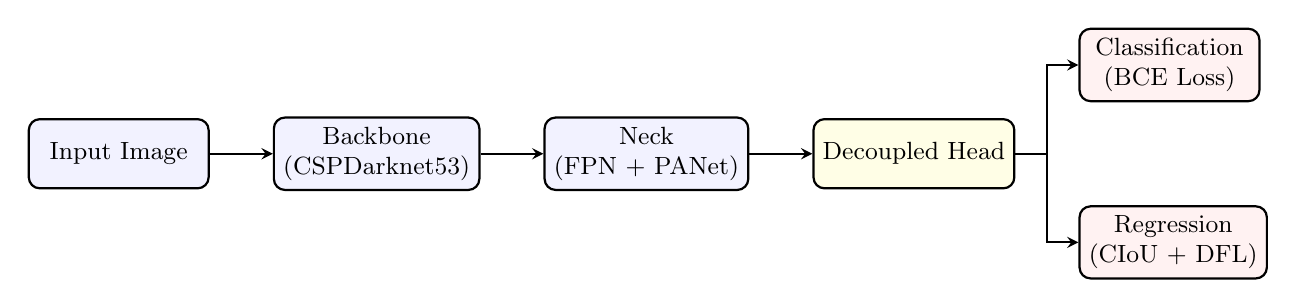
\begin{tikzpicture}[>=stealth, thick]
    \tikzset{
        block/.style={draw, fill=blue!5, rectangle, minimum height=2.5em, minimum width=6.5em, rounded corners, align=center, font=\small},
        split/.style={draw, fill=yellow!10, rectangle, minimum height=2.5em, minimum width=6.5em, rounded corners, align=center, font=\small},
        head/.style={draw, fill=red!5, rectangle, minimum height=2.5em, minimum width=6.5em, rounded corners, align=center, font=\small},
        line/.style={draw, ->, >=stealth, thick}
    }
    \node [block] (input) {Input Image};
    \node [block, right=0.8cm of input] (backbone) {Backbone\\(CSPDarknet53)};
    \node [block, right=0.8cm of backbone] (neck) {Neck\\(FPN + PANet)};
    \node [split, right=0.8cm of neck] (decoupled) {Decoupled Head};
    \node [head, above right=0.2cm and 0.8cm of decoupled] (cls) {Classification\\(BCE Loss)};
    \node [head, below right=0.2cm and 0.8cm of decoupled] (reg) {Regression\\(CIoU + DFL)};
    
    \path [line] (input) -- (backbone);
    \path [line] (backbone) -- (neck);
    \path [line] (neck) -- (decoupled);
    \draw [line] (decoupled.east) -- +(0.4,0) |- (cls.west);
    \draw [line] (decoupled.east) -- +(0.4,0) |- (reg.west);
\end{tikzpicture}
\end{document}